\section{Discussion}

In this discussion, the XFoil data is taken as "experimental" and the CFD data as numerical prediction; in addition, error bars of $\pm10\%$ were drawn from each XFoil data point. Observing the $C_l$ first in Fig. \ref{fig:error_bar1}, XFoil and CFD agree very well until separation, which CFD predicted to happen at a lower AoA. In this case, the CFD simulation might be more trustworthy, as it is difficult to predict separation, especially with low-fidelity methods. Regarding $C_d$, a separate figure, Fig \ref{fig:error_bar4}, more clearly illustrates the differences. The CFD generally overpredicted the XFoil solution. Near moderate AoAs of -5$^\circ$ to +5$^\circ$, the CFD prediction is about 10\% above that of XFoil; this was as close as the two solutions ever came. More extreme AoAs led to larger discrepancies, where the CFD predictions increasingly overpredicted the XFoil estimates. In general, the over estimate can at least partially be attributed to numerical diffusion of second order schemes. However, the discrepancy becomes larger with AoA which implies some correlation. It is this author's suspicion that both increasing suction near the leading edge and separation at the trailing edge may be impacting the fidelity of the CFD prediction.

\begin{figure}[H]
\centering
    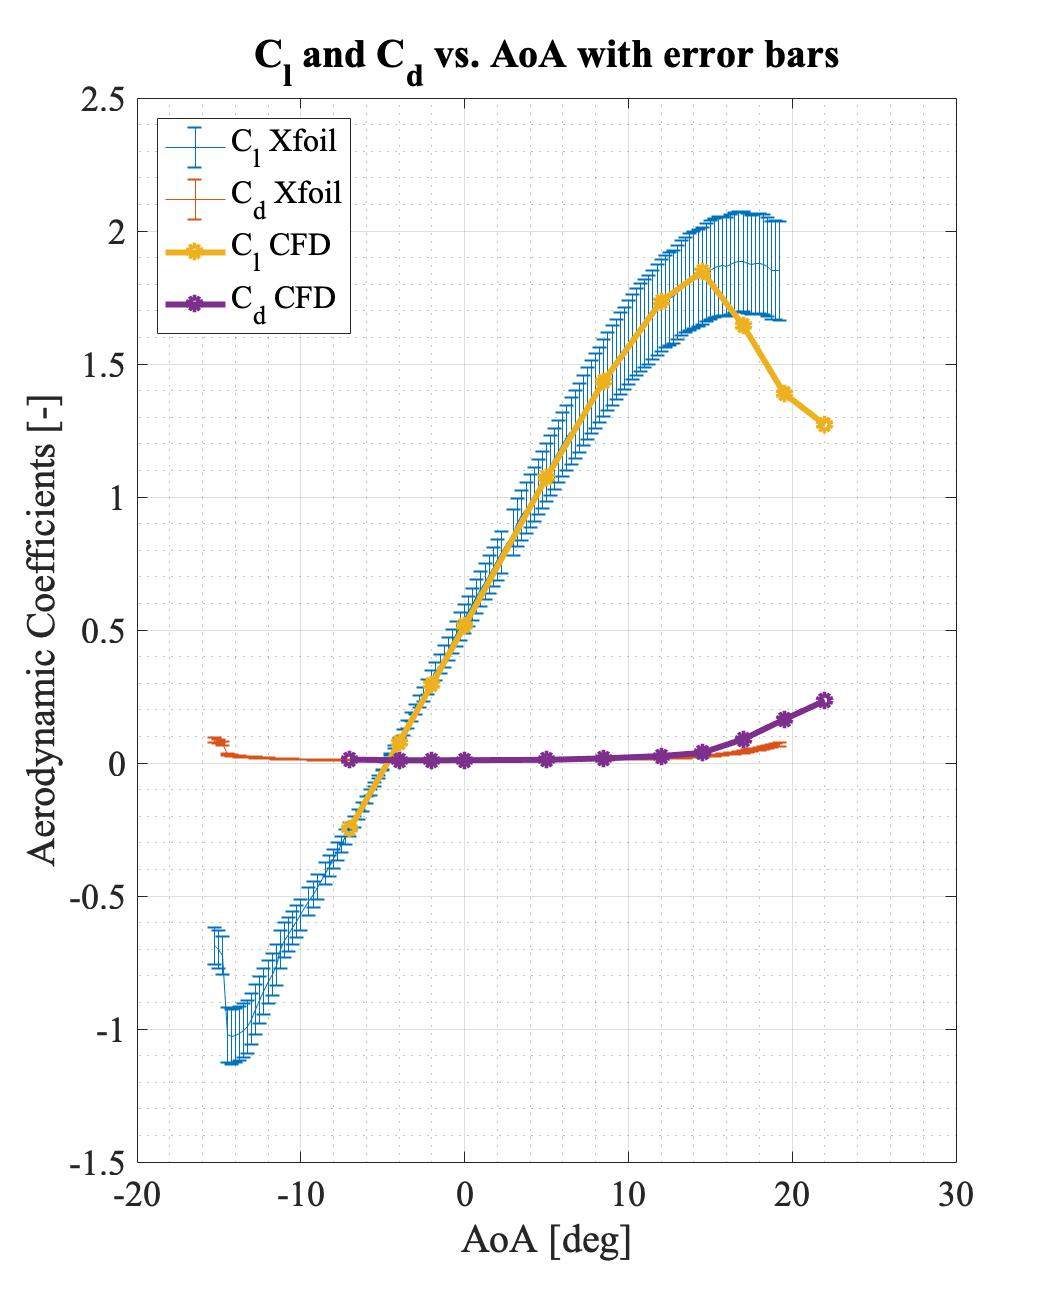
\includegraphics[width=0.65\textwidth]{error_bar1.jpg}
    \caption{$C_l$ and $C_d$ comparisons with error bars of $\pm$10\%}
    \label{fig:error_bar1}
\end{figure}

\begin{figure}[H]
\centering
    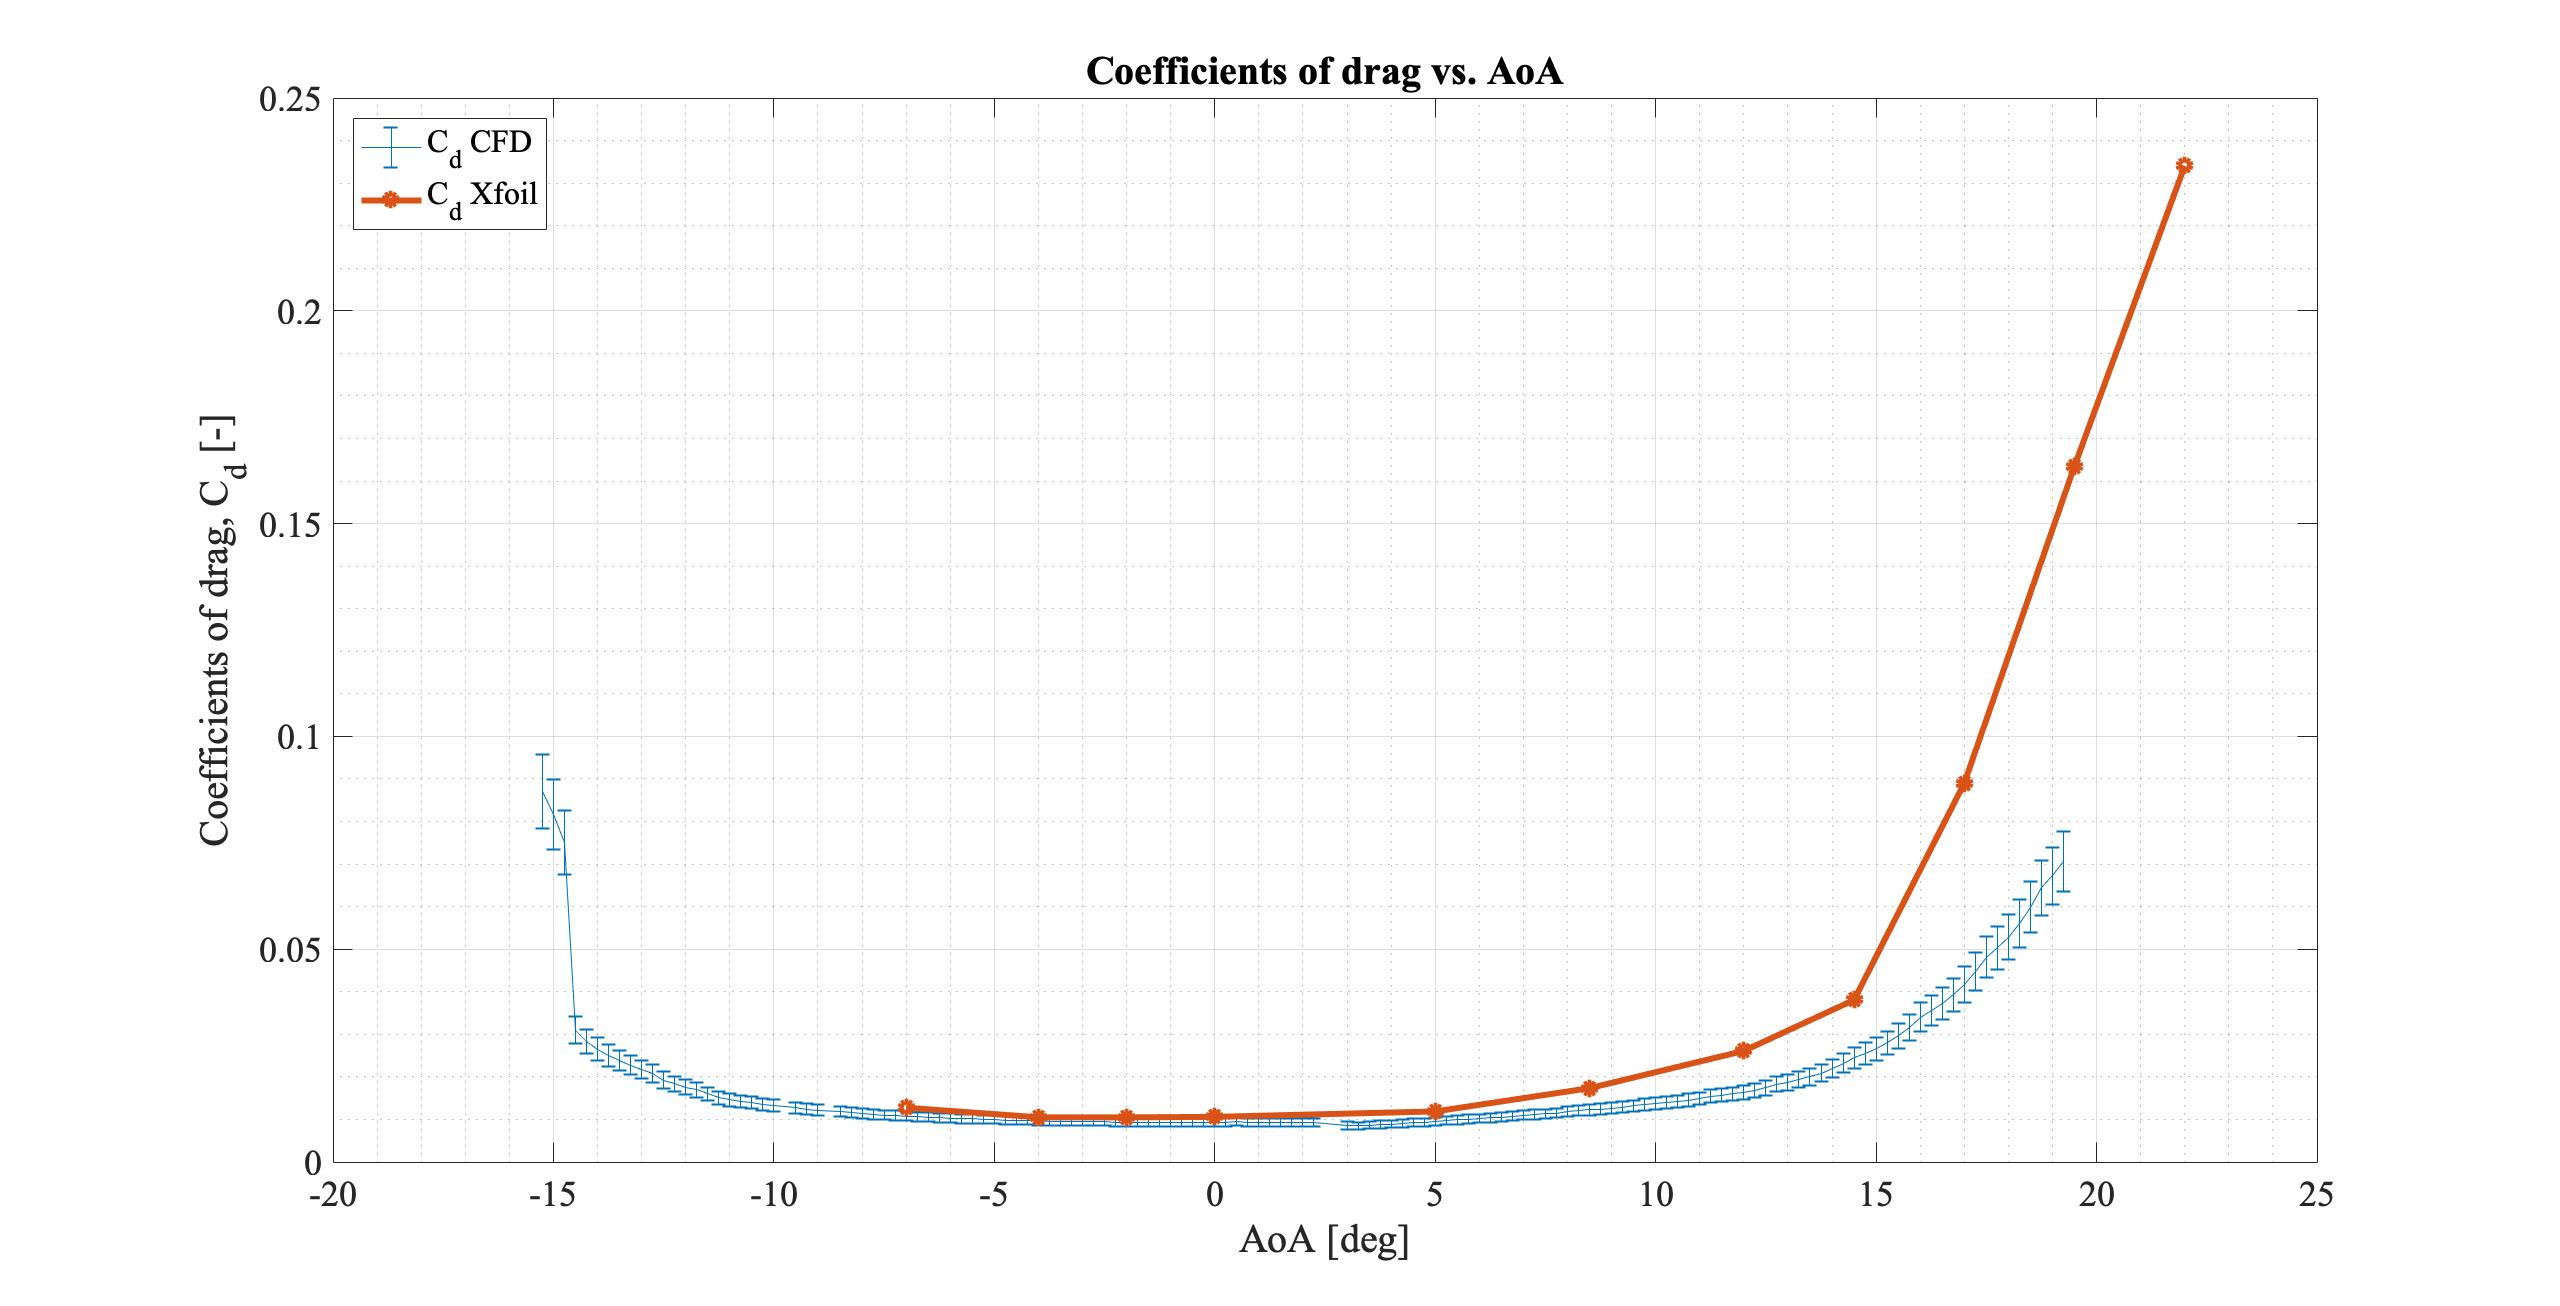
\includegraphics[width=\textwidth]{error_bar4.jpg}
    \caption{$C_d$ comparisons with error bar of $\pm$10\%}
    \label{fig:error_bar4}
\end{figure}

%\begin{figure}[H]
%  \begin{subfigure}[b]{0.5\textwidth}
%    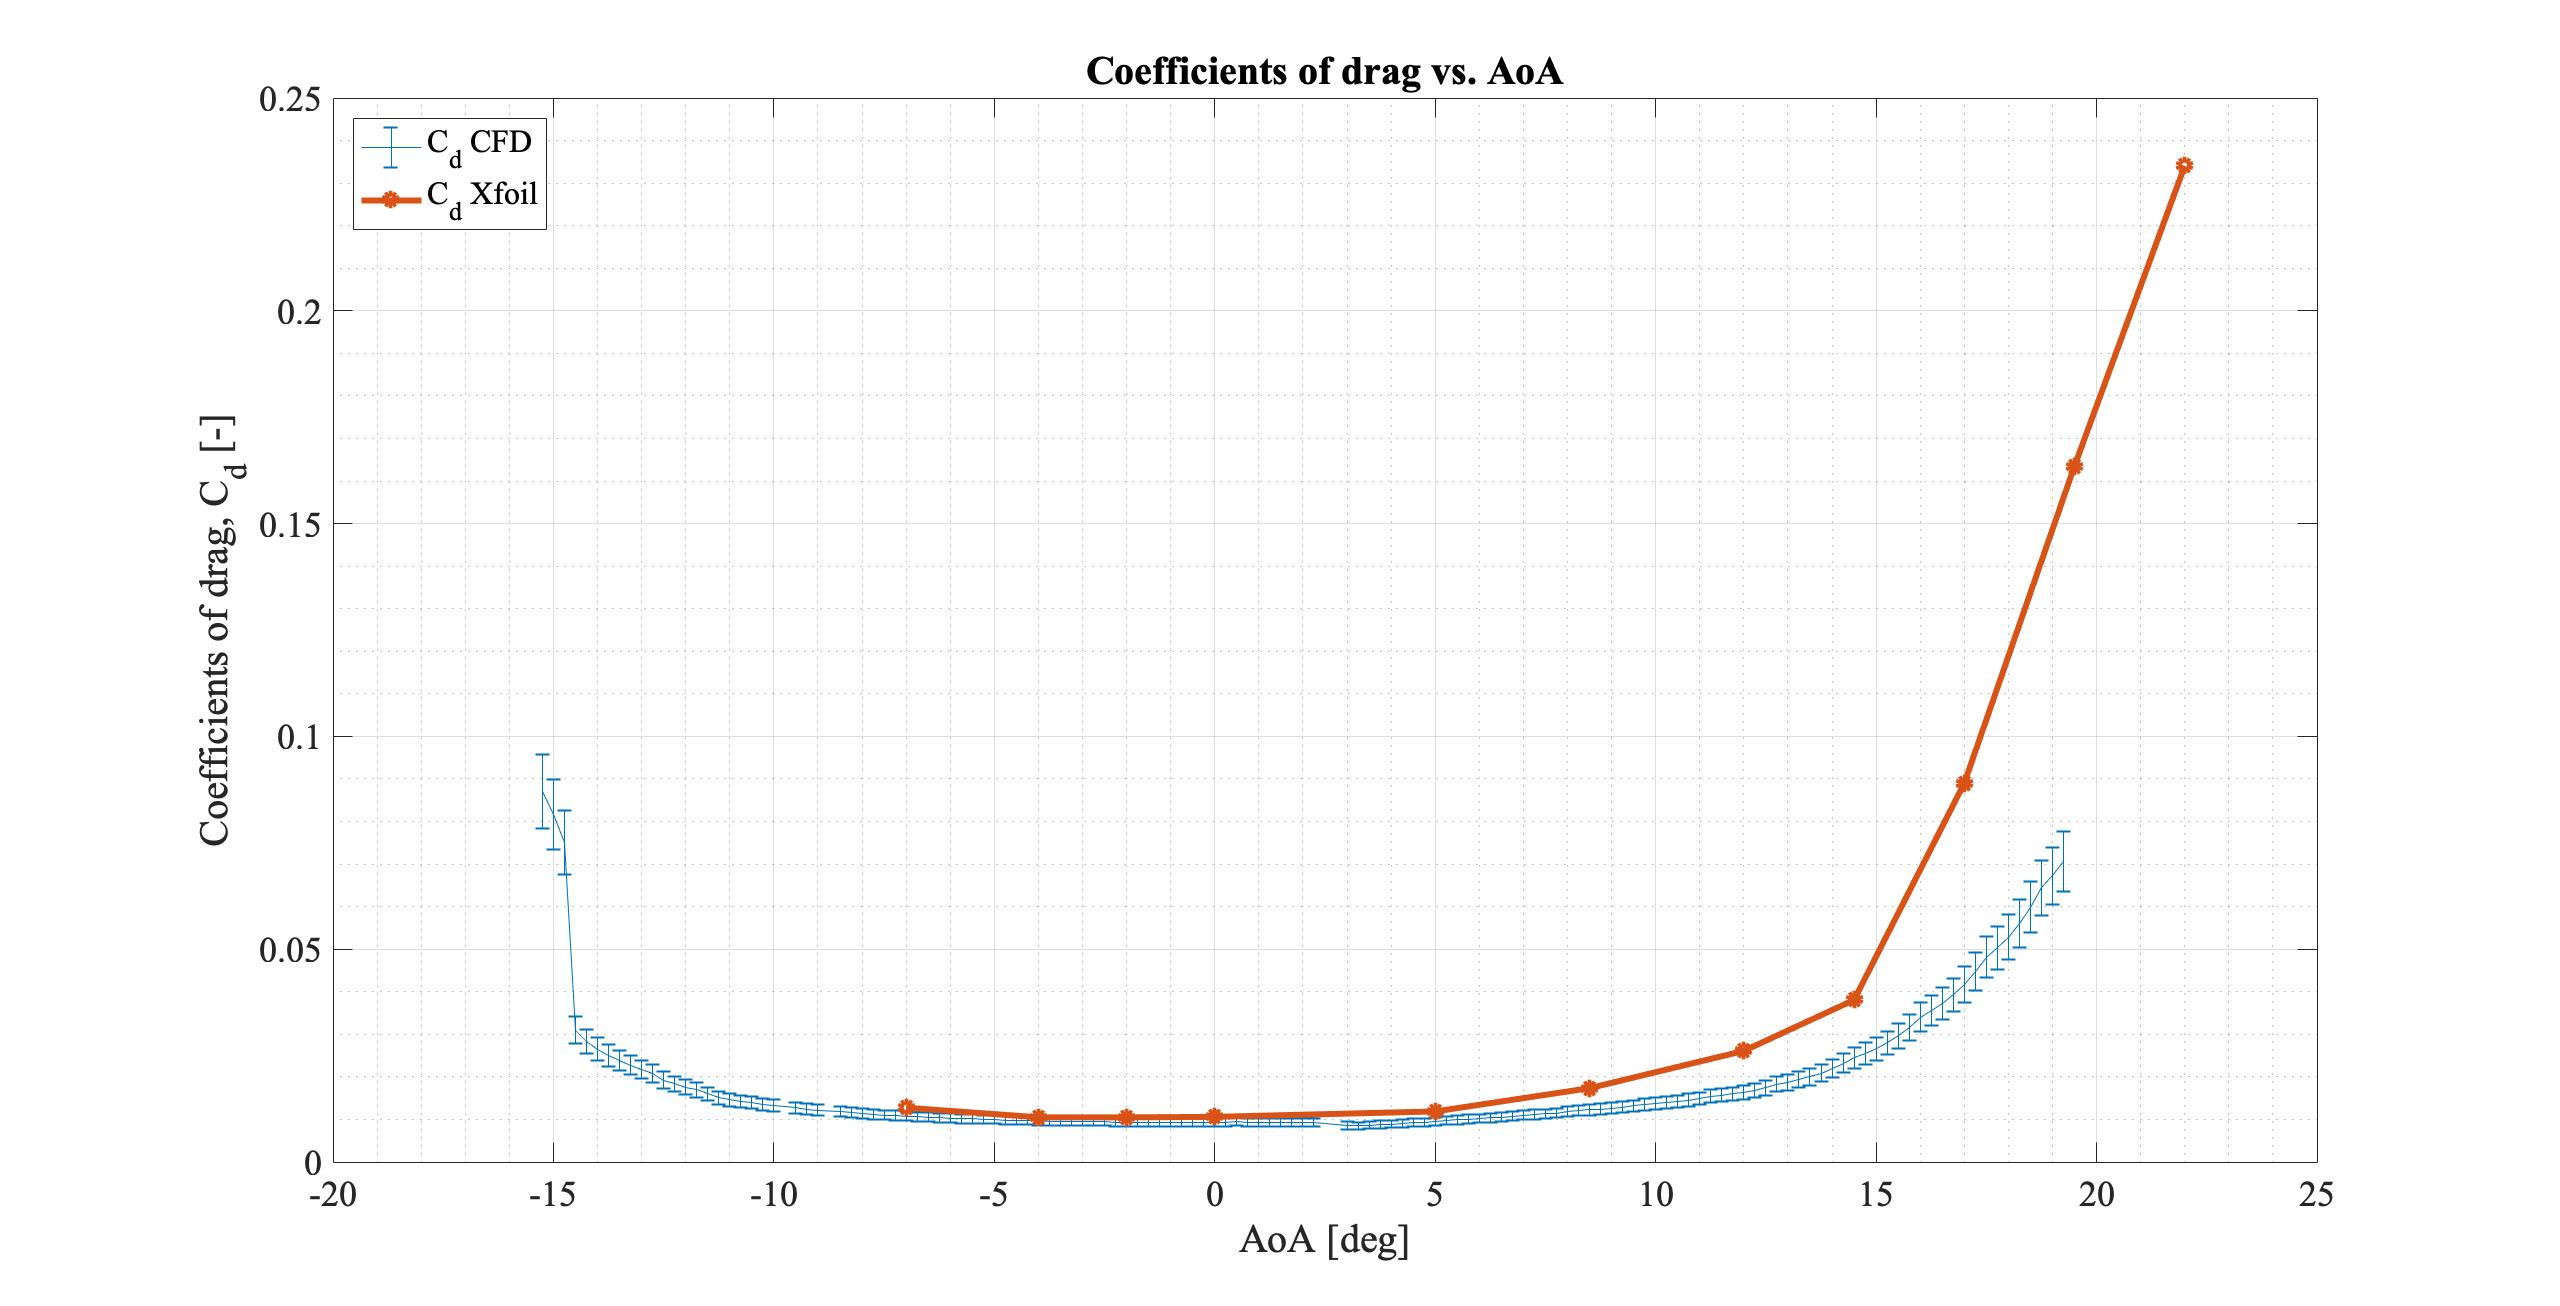
\includegraphics[width=\textwidth]{error_bar4.jpg}
%    \caption{$C_d$ comparison and error bar}
%    \label{fig:error_bar2}
%  \end{subfigure}
%  \begin{subfigure}[b]{0.5\textwidth}
%    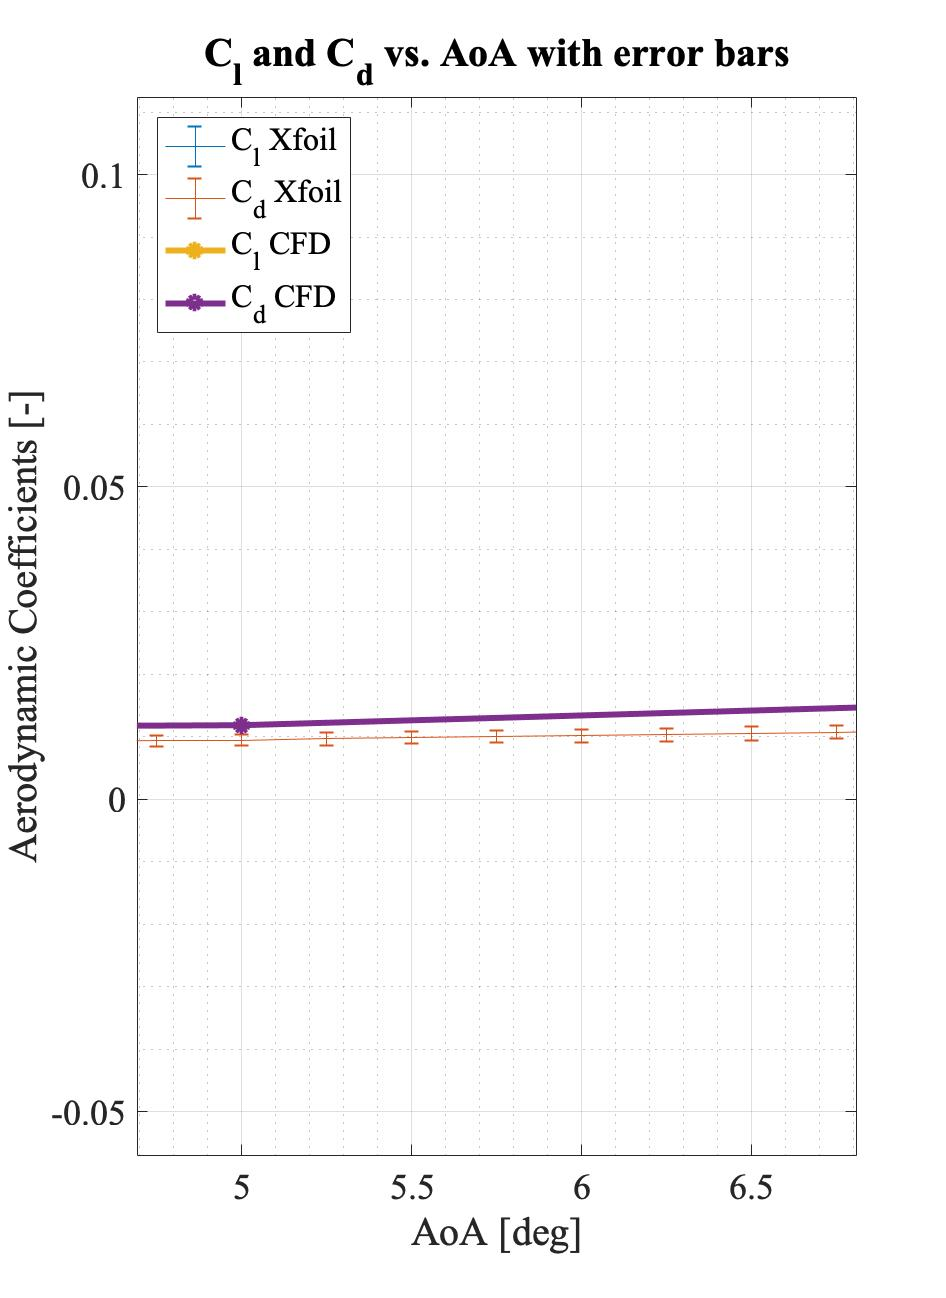
\includegraphics[width=\textwidth]{error_bar3.jpg}
%    \caption{Another zoomed-in view of larger AoA section of $C_d$}
%    \label{fig:error_bar3}
%  \end{subfigure}
%\end{figure}
